\begin{enumerate}[(a)]
    \item G 
    \begin{figure}[H]
    \centering
    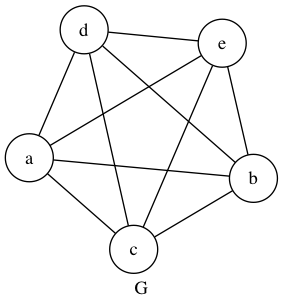
\includegraphics[scale=0.5]{115/115aG.png}
    \end{figure}
    H
    \begin{figure}[H]
    \centering
    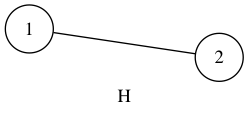
\includegraphics[scale=0.5]{115/115aH.png}
    \end{figure}
    $G+H$
    \begin{figure}[H]
    \centering
    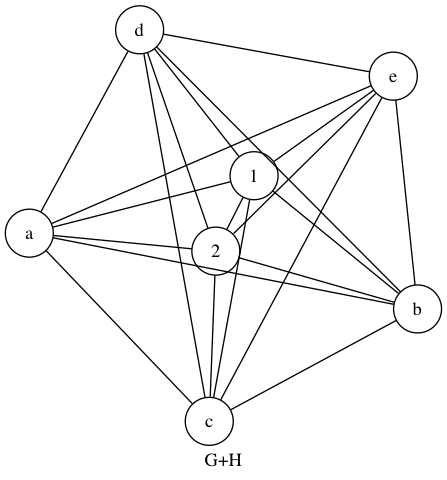
\includegraphics[scale=0.5]{115/115aGH.png}
    \end{figure}
    $G \times H$
    \begin{figure}[H]
    \centering
    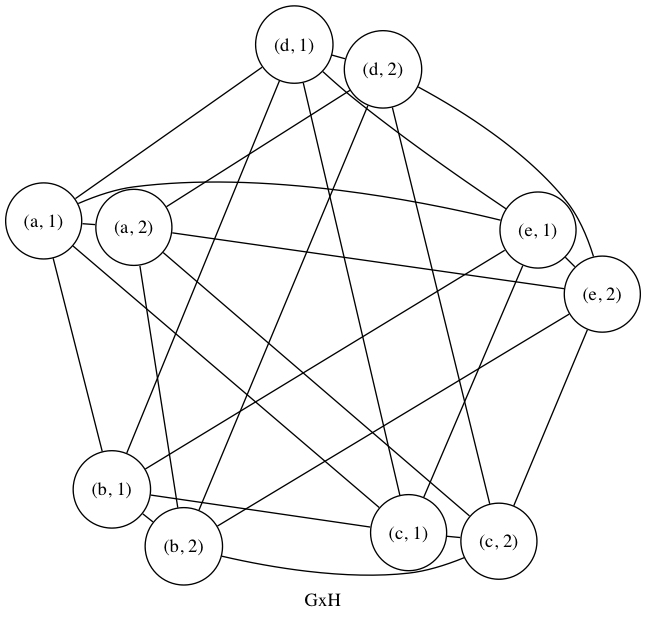
\includegraphics[scale=0.5]{115/115aGH2.png}
    \end{figure}


    \item G 
    \begin{figure}[H]
    \centering
    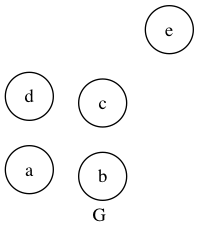
\includegraphics[scale=0.5]{115/115bG.png}
    \end{figure}
    H
    \begin{figure}[H]
    \centering
    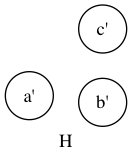
\includegraphics[scale=0.5]{115/115bH.png}
    \end{figure}
    $G+H$
    \begin{figure}[H]
    \centering
    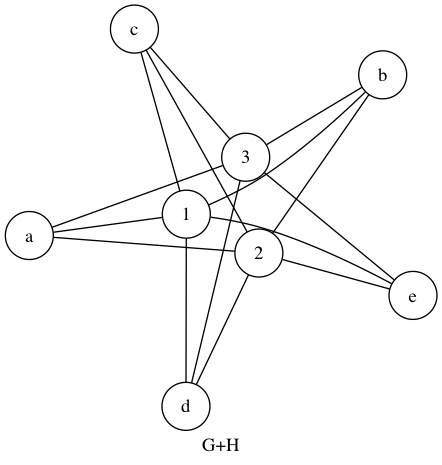
\includegraphics[scale=0.5]{115/115bGH.png}
    \end{figure}
    $G \times H$
    \begin{figure}[H]
    \centering
    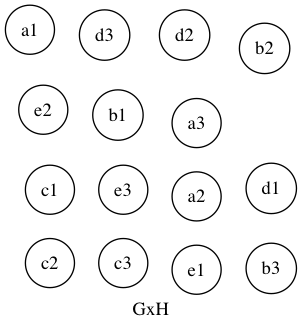
\includegraphics[scale=0.5]{115/115bGH2.png}
    \end{figure}

    \item G 
    \begin{figure}[H]
    \centering
    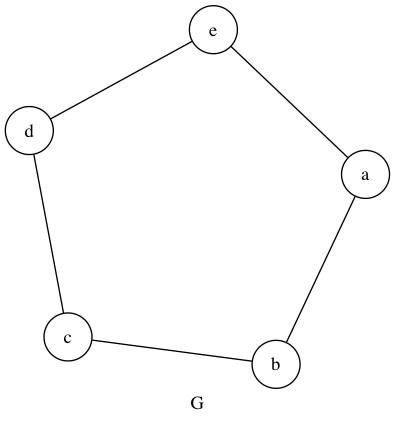
\includegraphics[scale=0.5]{115/115cG.png}
    \end{figure}
    H
    \begin{figure}[H]
    \centering
    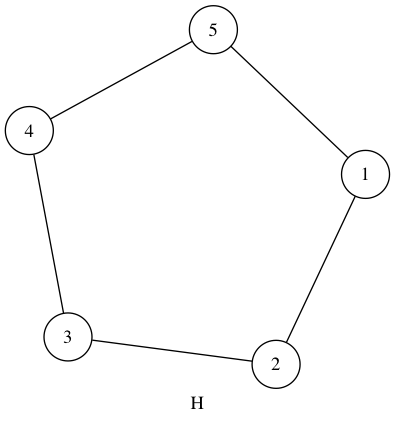
\includegraphics[scale=0.5]{115/115cH.png}
    \end{figure}
    $G+H$
    \begin{figure}[H]
    \centering
    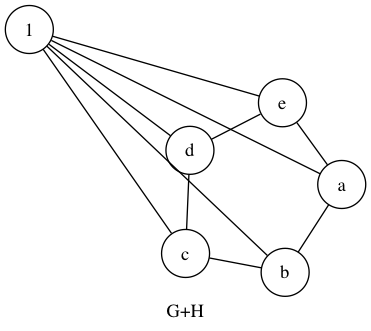
\includegraphics[scale=0.5]{115/115cGH.png}
    \end{figure}
    $G \times H$
    \begin{figure}[H]
    \centering
    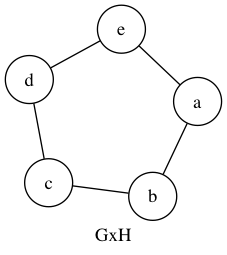
\includegraphics[scale=0.5]{115/115cGH2.png}
    \end{figure}
\end{enumerate}
